% 	 1) Картинки с захватом и распределением по E,L
%		вначале и в конце эволюции (100 GeV, 100 KeV)
%	 2) Картинки для Скорости захвата и аннигиляции 
%		C(delta) и A(delta) с учётом аннигиляции и без %		учёта аннигиляции, сравнение с tan^2()
%	 3) Коэффициент аннигиляции a как функция от delta %		и m
%	 4) Графики в плоскости M,delta где есть равновесие	
%    

Изобразим распределение частиц по энергии и моменту импульса (на единицу массы частицы). Мы будем отсчитывать энергию и момент в безразмерных единицах. Безразмерные энергия и момент импульса соответственно равны:
\begin{equation}
	\begin{split}
		E = \cfrac{\frac{1}{2} v_{\chi}^2 + \phi(r)}
		{\frac{1}{2} v_{esc}^2} \\
		L = \cfrac{|\vec{r} \times \vec{v}|}
		{R_{\odot} v_{esc}}
	\end{split}
\end{equation}

Еще одна величина --- приведенный момент импульса.
\begin{equation}
	l = \cfrac{L}{L_{max}(E)}
\end{equation}

где $L_{max}(E)$ --- максимально возможный момент импулься траектории при данной энергии (не учитываются траектории, которые находятся вне Солнца).

Мы будем рассматривать распределение частиц по энергтт и приведеному импульсу $f(E,l) = \frac{dN}{dE dl}$.

\begin{figure}[ht]
	\centering
	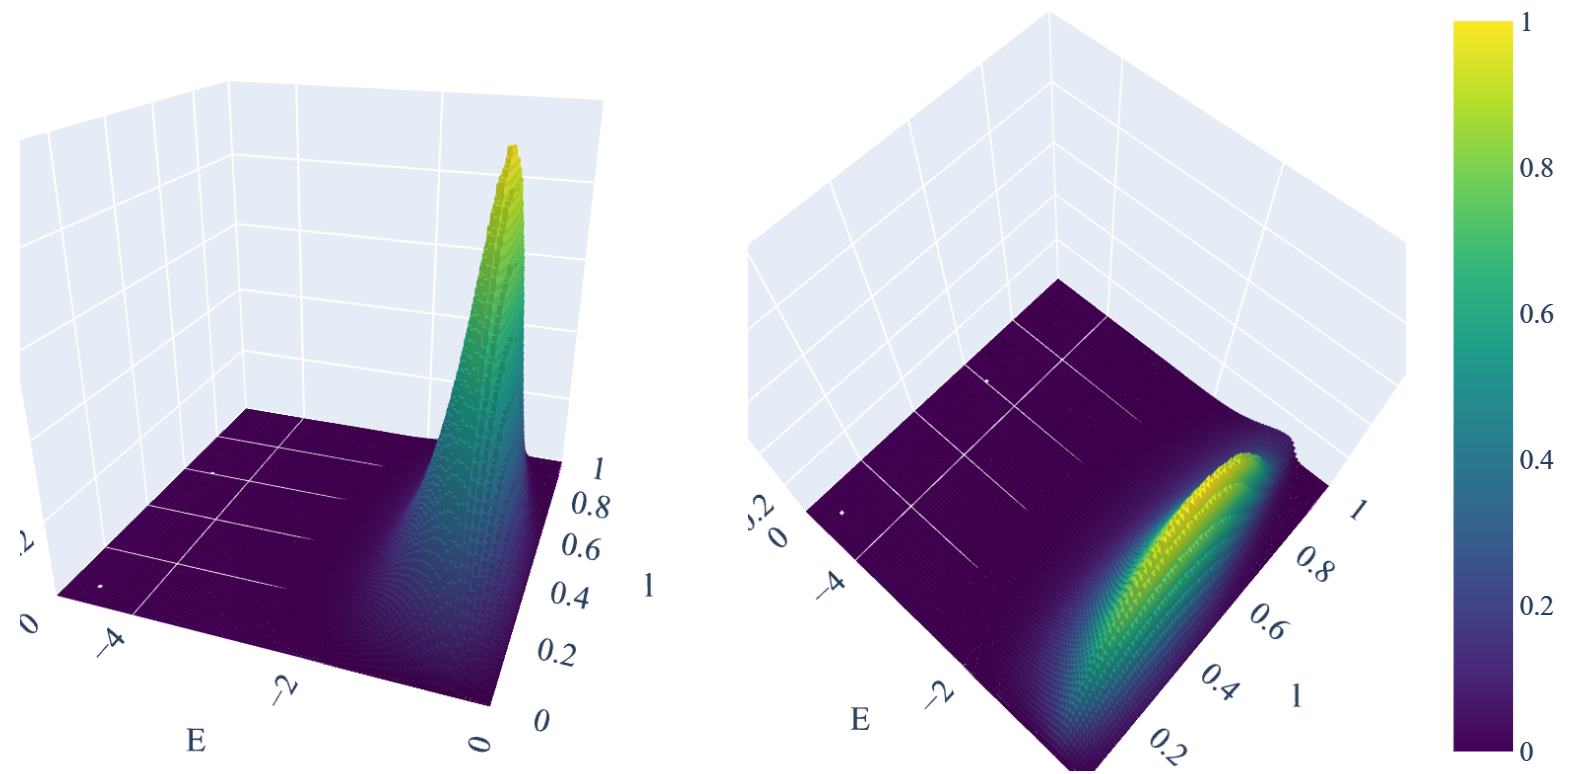
\includegraphics[width=0.7\textwidth]
	{images/Capt100_100.png}
	\caption{Распределение захваченных частиц для $m_{\chi} = 100\, \text{GeV}$, $\delta = 100\, \text{keV}$.}
	\label{fig:Capt100_100}
\end{figure}

\begin{figure}[!h]
	\centering
	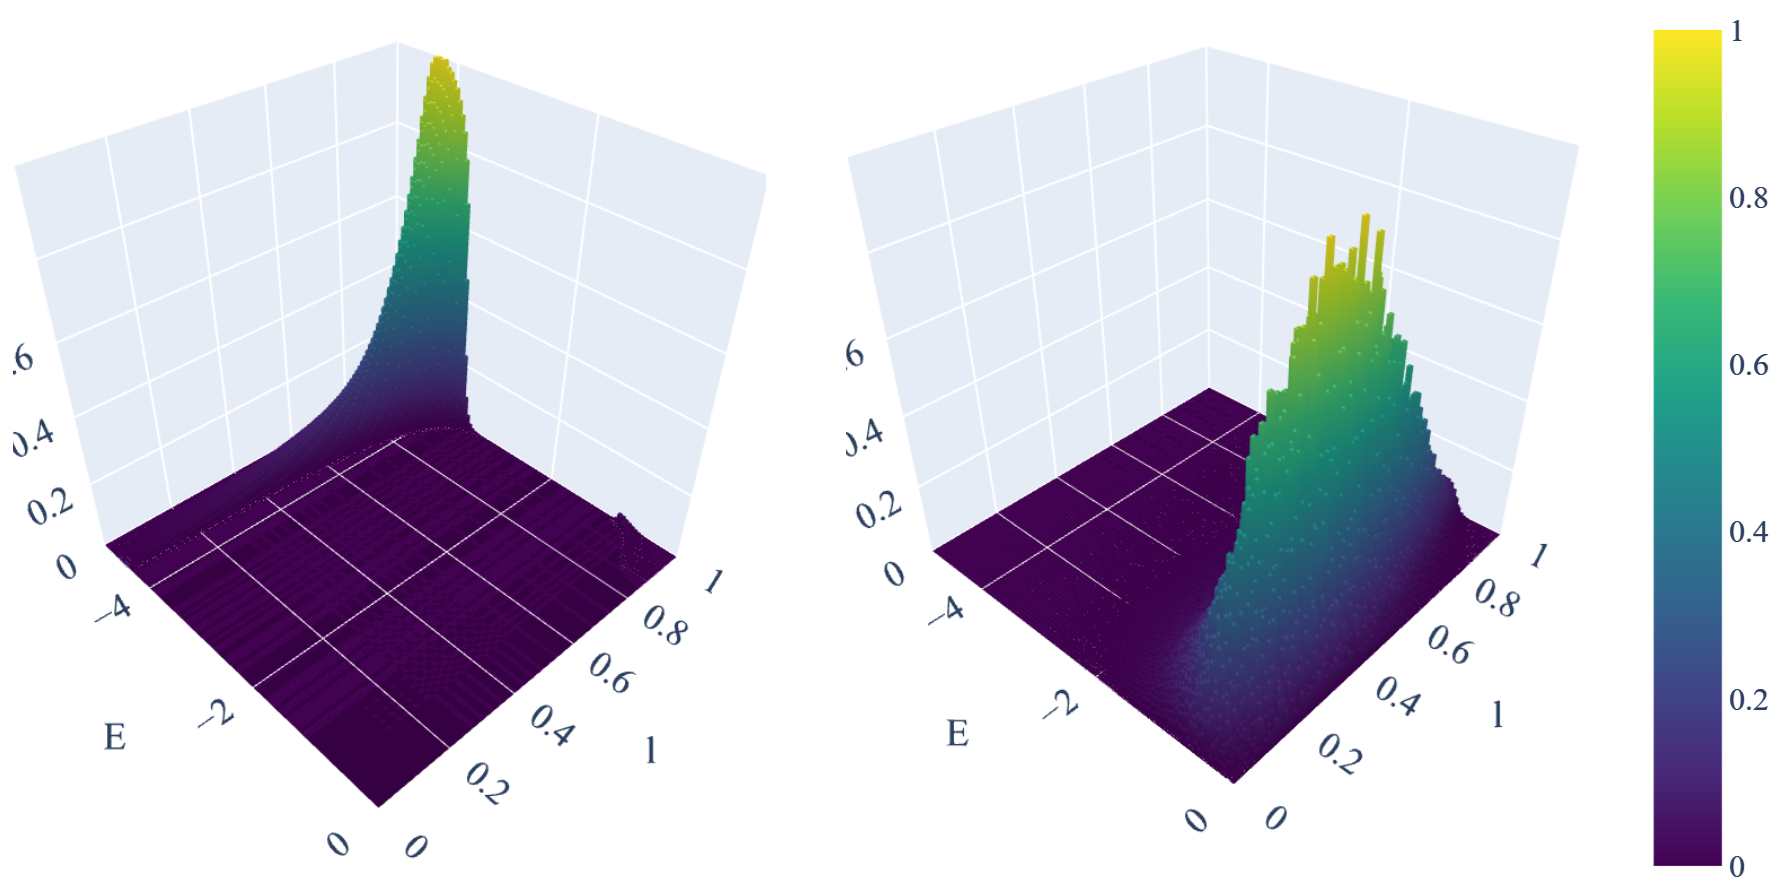
\includegraphics[width=0.7\textwidth]
	{images/Dout100_100.png}
	\caption{Распределение частиц в конце эволюции для $m_{\chi} = 100\, \text{GeV}$, $\delta = 100\, \text{keV}$.}
	\label{fig:Dout100_100}
\end{figure}

\begin{figure}[!h]
\centering
\begin{tikzpicture}
	\begin{axis}[
		%title = {Распределение по $r/R_{\odot}$},
		no markers,
		xmin=0,
		xmax=0.2,
		xtick distance=0.02,
		 xticklabel style={
			/pgf/number format/fixed
		},
		xlabel = \(r\),
		ylabel = {\(\cfrac{d^3N}{d^3r}\)},
		table/col sep = semicolon,
		height = 0.2\paperheight, 
		width = 0.8\paperwidth,
		/pgf/number format/1000 sep={}
		]
		\addplot table [mark=none, x={R}, y={D100}]{tables/CaptDout100_100and50.csv};
		\addplot table [mark=none, x={R}, y={D50}]{tables/CaptDout100_100and50.csv};
		\addplot table [mark=none, x={R}, y={C100}]{tables/CaptDout100_100and50.csv};
		\addplot table [mark=none, x={R}, y={C50}]{tables/CaptDout100_100and50.csv};
		\addplot table [mark=none, x={R}, y={N}]{tables/Term100.csv};
		\legend{ 
			{$N(T_{\odot})$, $\delta = 100\text{keV}$},
			{$N(T_{\odot})$, $\delta = 50\text{keV}$},
			{$C$, $\delta = 100\text{keV}$},
			{$C$, $\delta = 50\text{keV}$},
			{$N_{therm}$}			
		};
	\end{axis}
\end{tikzpicture}
	\caption{Концентраця частиц тёмной материи массы $m_{\chi} = 100\text{GeV}$}
	\label{eq:Nrdistrib}
\end{figure}

Главный вопрос заключается в отношении скорости аннигиляции и скорости захвата $C/A$. Мы рассматриваем уравнение эволюции как с учётом аннигиляции так и без учета аннигиляции. 

\begin{figure}[!h]
	\centering
	\begin{tikzpicture}
		\begin{axis}[
			%title = {Распределение по $r/R_{\odot}$},
			no markers,
			xlabel = {$\delta$, $\text{keV}$},
			ylabel = {Rate, $\frac{1}{\text{s}}$},
			ymode=log,
			table/col sep = semicolon,
			height = 0.2\paperheight, 
			width = 0.8\paperwidth,
			/pgf/number format/1000 sep={}
			]
			\addplot table [mark=none, x={dM}, y={C}]{tables/CaptAnn_noAnn100.csv};
			
			\addplot table [mark=none, x={dM}, y={A}]{tables/CaptAnn_noAnn100.csv};
			
			\addplot table [mark=none, x={dM}, y={A}]{tables/Ann_withAnn100.csv};
			
			\addplot table [mark=none, x={dM}, y={Ath}]{tables/CaptAnn_noAnn100.csv};
			\legend{ 
				{Capture},
				{$A$, linear},
				{$A$, nonlinear},
				{$A = C \th^2{\sqrt{at^2C}}$}
			};
		\end{axis}
	\end{tikzpicture}
	\caption{Зависимость от $\delta$ захвата и аннигиляции при линейной и нелинейной эволюции для $m_{\chi} = 100\text{GeV}$}
	\label{eq:CaptAnn}
\end{figure}

Как можно заметить, если включить в уравнение эволюции аннигиляцию, то результат совпадает с оценкой (\ref{eq:AnnNtherm}). 



